\begin{tikz*}[%
	every node/.style={align=center},
	border/.style={rectangle,thick,draw=red,font=\color{red}},
	label/.style={font=\color{red}\small,fill=white}
]
	\node(a) {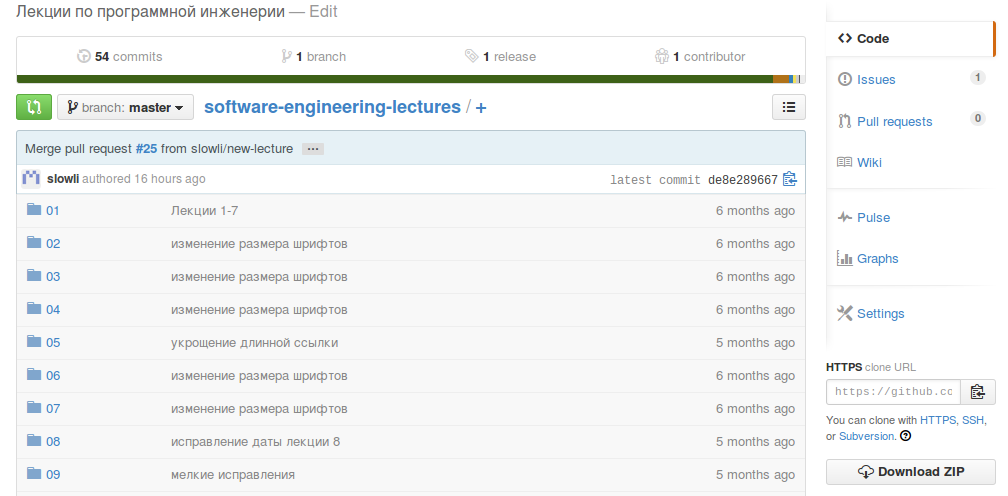
\includegraphics[scale=0.4]{fig-github.png}};

	\node<2> at (-4em,-2.75em) [border,minimum width=35em,minimum height=16em] {%
		\Large{Список файлов} \\ (для просомотра и редактирования)};

	\node<3>(commits) at (-16.5em,8.25em) [border,minimum width=6.5em,minimum height=1.5em] {};
	\node<3> [label,below=0pt of commits] {операции фиксации \\ в текущей ветви};

	\node<4>(branch) at (-16.25em,6em) [border,minimum width=6.5em,minimum height=1.5em] {};
	\node<4> [label,below=0pt of branch] {выбор ветви};

	\node<5>(release) at (0em,8.25em) [border,minimum width=6.5em,minimum height=1.5em] {};
	\node<5> [label,below=0pt of release] {создание и \\ скачивание выпусков};

	\node<6>(issue) at (17.5em,7.35em) [border,minimum width=7.5em,minimum height=1.5em] {};
	\node<6> [label,below=0pt of issue,anchor=north east] {работа с запросами \\ на изменение};

	\node<7>(url) at (17.5em,-5.75em) [border,minimum width=8.5em,minimum height=2.5em] {};
	\node<7> [label,above=0pt of url,anchor=south east] {ссылка для \\ клонирования};

	\node<8>(download) at (17.5em,-9.65em) [border,minimum width=8.5em,minimum height=1.5em] {};
	\node<8> [label,above=0pt of download,anchor=south east] {скачивание основной \\ версии репозитория};
\end{tikz*}
